% Commandes pour représenter des compoants avec tikz
\newcommand\ammeter{to node[draw,circle,fill=black!10] {{\bf A}}}    			% ampèremètre
\newcommand\voltmeter{to node[draw,circle,fill=black!10] {{\bf V}}}  			% voltmètre
\newcommand\generateur[1][fill=black!10]{to node[draw,circle, #1] {{\bf G}}}	% générateur
\newcommand\moteur[1][black!10]{to node[draw,circle,fill=#1] {{\bf M}}} 		% moteur
\newcommand\dipole[1]{to node[draw, circle, fill=white] {{\bf #1}}}				% dipôle générique
\newcommand\dipolegris[1]{to node[draw, circle, fill=\docbkg] {{\bf #1}}}		% dipôle rempli avec la couleur de fond des documents



% Représenter une masse sur un schéma
% Usage :
%	\draw (x,y) \masse;
\newcommand\masse{node {
	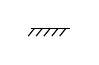
\begin{tikzpicture}
		\draw (-0.25,0) -- (0.25,0);
		\foreach \x in {-0.2, -0.1, ..., 0.2}{
			\draw (\x,0) --++ (-0.08,-0.1);
		}
	\end{tikzpicture}
}}

% Représenter une masse vers le haut
% Usage :
%	\draw (x,y) \masseup;
\newcommand\masseup{node[rotate=180] {
	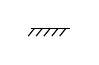
\begin{tikzpicture}
		\draw (-0.25,0) -- (0.25,0);
		\foreach \x in {-0.2, -0.1, ..., 0.2}{
			\draw (\x,0) --++ (-0.08,-0.1);
		}
	\end{tikzpicture}
}}



% Flèches en rouge pour le courant électrique
\makeatletter
\ctikzset{current arrow color/.initial=black} % create key

\pgfdeclareshape{currarrow}{
    \anchor{center}{
        \pgfpointorigin
    }
        \anchor{tip}{
        \pgfpointorigin
            \pgf@circ@res@step = \pgf@circ@Rlen
                \divide \pgf@circ@res@step by 16
        \pgf@x  =\pgf@circ@res@step
        }
    \behindforegroundpath{

        \pgfscope
            \pgf@circ@res@step = \pgf@circ@Rlen
            \divide \pgf@circ@res@step by 16

            \pgfpathmoveto{\pgfpoint{-.7\pgf@circ@res@step}{0pt}}
            \pgfpathlineto{\pgfpoint{-.7\pgf@circ@res@step}{-.8\pgf@circ@res@step}}
            \pgfpathlineto{\pgfpoint{1\pgf@circ@res@step}{0pt}}
            \pgfpathlineto{\pgfpoint{-.7\pgf@circ@res@step}{.8\pgf@circ@res@step}}
            \pgfpathlineto{\pgfpoint{-.7\pgf@circ@res@step}{0pt}}
            \pgfsetcolor{\pgfkeysvalueof{/tikz/circuitikz/current arrow color}}
            \pgfusepath{draw,fill}
        \endpgfscope
    }
}
\makeatother

\tikzstyle{elec}=[circuitikz/current arrow color=red]